다음 그림에서 점 $\mathrm{O}$는 $\angle\mathrm{A} = 90^\circ$ 인 직각삼각형 $\mathrm{ABC}$의 빗변 $\mathrm{BC}$의 중점이다. $\angle\mathrm{ABC} = 46^\circ$ 일 때, $\angle x$의 크기는 몇 도인지 구하여라.

\begin{figure}[h]
\centering
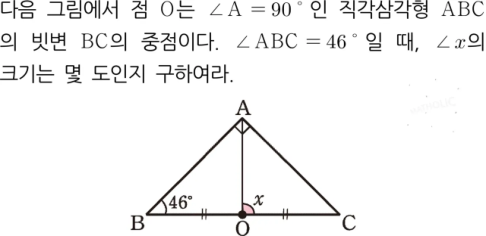
\includegraphics[width=0.3\textwidth]{plain0_problem_06_figure.png}
\end{figure}
